\section{Appendix}
\subsection{Discrete Fourier Series (DFS)}
Complex exponential Fourier series synthesis and analysis equations for a periodic discrete-time signal having period $p$ :
\[
    x(n)=\sum_{k=\langle p\rangle} X_k e^{i k \omega_0 n} \quad \longleftrightarrow \quad X_k=\frac{1}{p} \sum_{n=\langle p\rangle} x(n) e^{-i k \omega_0 n},
\]
where $\omega_0=\frac{2 \pi}{p}$ and $\langle p\rangle$ denotes a suitable discrete interval of length $p$ (i.e., an interval containing $p$ contiguous integers). For example, $\sum_{k=\langle p\rangle}$ may denote $\displaystyle\sum_{k=0}^{p-1} \text { or } \sum_{k=1}^p .$

\subsection{Continuous-Time Fourier Series (FS)}
Complex exponential Fourier series synthesis and analysis equations for a periodic continuous-time signal having period $p$:
$$
x(t)=\sum_{k=-\infty}^{\infty} X_k e^{i k \omega_0 t} \quad \longleftrightarrow \quad X_k=\frac{1}{p} \int_{\langle p\rangle} x(t) e^{-i k \omega_0 t} d t
$$
where $\omega_0=\frac{2 \pi}{p}$ and $\langle p\rangle$ denotes a suitable continuous interval of length $p$. For example, $\displaystyle\int_{\langle p\rangle}$ can denote $\displaystyle\int_0^p$.

\subsection{Transfer Function and Frequency Response of a DT LTI System}
Consider a real, discrete-time LTI system having impulse response $h: \mathbb{Z} \rightarrow \mathbb{R}$. The transfer function $\widehat{H}: \mathbb{C} \rightarrow \mathbb{C}$ of the system is given by:
$$
\widehat{H}(z)=\sum_{n=-\infty}^{\infty} h(n) z^{-n}, \quad \forall z \in \operatorname{RoC}(h) .
$$
If the system is stable, its frequency response $H: \mathbb{R} \rightarrow \mathbb{C}$ is given by:
$$
H(\omega)=\sum_{n=-\infty}^{\infty} h(n) e^{-i \omega n}, \quad \forall \omega \in \mathbb{R} .
$$
The impulse response of the system is given by:
$$
h(n)=\frac{1}{2 \pi} \int_{\langle 2 \pi\rangle} H(\omega) e^{i \omega n} d \omega .
$$

% \newpage
\subsection{Transfer Function and Frequency Response of a CT LTI System}
Consider a real, continuous-time LTI system having impulse response $h: \mathbb{R} \rightarrow \mathbb{R}$.
If the system is stable, its frequency response $H: \mathbb{R} \rightarrow \mathbb{C}$ is given by:
$$
H(\omega)=\int_{-\infty}^{\infty} h(t) e^{-i \omega t} d t, \quad \forall \omega \in \mathbb{R} .
$$
The impulse response of the system is given by:
$$
h(t)=\frac{1}{2 \pi} \int_{-\infty}^{\infty} H(\omega) e^{i \omega t} d \omega .
$$

\newpage
\subsection{Properties of the DTFT}
\[
    \boxed{
        x(n)=\frac{1}{2 \pi} \int_{\langle 2 \pi\rangle} X(\omega) e^{i \omega n} d \omega \longleftrightarrow X(\omega)=\sum_{n=-\infty}^{\infty} x(n) e^{-i \omega n}
    }
\]
% \hrulefill
\begin{table}[ht]
  \renewcommand*{\arraystretch}{1.2}
   \centering
  \resizebox{\columnwidth}{256px}{
    \begin{tabular}{|c|c|}
    \hline \textbf{Time domain} & \textbf{Frequency domain} \\
        \hline\makecell{$\forall n \in \mathbb{Z}, \quad x(n)$ is real\\\ } & \makecell{$\forall \omega \in \mathbb{R}, \quad X(\omega)=X^*(-\omega)$\\\ } \\
        \hline\makecell{$\forall n \in \mathbb{Z}, \quad x(n)=x^*(-n)$\\\ } & \makecell{$\forall \omega \in \mathbb{R}, \quad X(\omega)$ is real\\\ } \\
        \hline\makecell{\\$\forall n \in \mathbb{Z}, \quad y(n)=x(n-N)$\\\ } 
        & \makecell{\\$\forall \omega \in \mathbb{R}, \quad Y(\omega)=e^{-i \omega N} X(\omega)$\\\ } \\
        \hline\makecell{\\$\forall n \in \mathbb{Z}, \quad y(n)=e^{i \omega_1 n} x(n)$\\\ } 
        & $\forall \omega \in \mathbb{R}, \quad Y(\omega)=X\left(\omega-\omega_1\right)$ \\
        \hline\makecell{\\$\forall n \in \mathbb{Z}$, \\
        $y(n)=\cos \left(\omega_1 n\right) x(n)$\\\ } 
        & \makecell{\\$\forall \omega \in \mathbb{R}$, \\
        $Y(\omega)=\left(X\left(\omega-\omega_1\right)+X\left(\omega+\omega_1\right)\right) / 2$\\\ } \\
        \hline\makecell{\\$\forall n \in \mathbb{Z}$, \\
        $y(n)=\sin \left(\omega_1 n\right) x(n)$\\\ } 
        & \makecell{\\$\forall \omega \in \mathbb{R}$,\\ $Y(\omega)=\left(X\left(\omega-\omega_1\right)-X\left(\omega+\omega_1\right)\right) / {2 i}$\\\ } \\
        \hline\makecell{\\$\forall n \in \mathbb{Z}$, \\ $x(n)=a x_1(n)+b x_2(n)$\\\ } & \makecell{\\$\forall \omega \in \mathbb{R}$ \\ $X(\omega)=a X_1(\omega)+b X_2(\omega)$\\\ }\\
        \hline\makecell{\\$\forall n \in \mathbb{Z}, \quad y(n)=(h * x)(n)$\\\ } & \makecell{\\$\forall \omega \in \mathbb{R}, \quad Y(\omega)=H(\omega) X(\omega)$\\\ } \\
        \hline
        \makecell{$\forall n \in \mathbb{Z}, \quad y(n)=x(n) p(n)$\\\ } & \makecell{\\$\forall \omega \in \mathbb{R}$,\\
        $Y(\omega)=\frac{1}{2 \pi} \int_0^{2 \pi} X(\Omega) P(\omega-\Omega) d \Omega$\\\ }
        \\
        \hline
        \makecell{\\$\forall n \in \mathbb{Z},$\\ 
            $y(n)=$ 
            $\begin{cases}x(n / N) & n \text { is a multiple of } N \\ 0 & \text { otherwise }\end{cases}$
            \\\ 
        }
        & \makecell{$\forall \omega \in \mathbb{Z}$, 
            \\
            $Y(\omega)=X(N \Omega)$
        }
        \\
        \hline
    \end{tabular}
  }
\end{table}

\newpage
\subsection{Properties of the CTFT}
\begin{table}[ht]
  \renewcommand*{\arraystretch}{1.2}
   \centering
  \resizebox{400px}{256px}{
    \begin{tabular}{|c|c|}
    \hline \textbf{Time domain} & \textbf{Frequency domain} \\
        \hline
        \makecell{$\forall t \in \mathbb{R}, \quad x(t)$ is real} 
            & \makecell{$\forall \omega \in \mathbb{R}, \quad X(\omega)=X^*(-\omega)$} 
            \\
        \hline
        \makecell{\\$\forall t \in \mathbb{R}, \quad x(t)=x^*(-t)$\\\ } 
            & \makecell{\\$\forall \omega \in \mathbb{R}, \quad X(\omega)$ is real\\\ } 
            \\
        \hline
        \makecell{\\$\forall t \in \mathbb{R}, \quad y(t)=x(t-\tau)$\\\ } 
            & \makecell{\\$\forall \omega \in \mathbb{R}, \quad Y(\omega)=e^{-i \omega\tau} X(\omega)$\\\ } 
            \\
        \hline
        \makecell{\\$\forall t \in \mathbb{R}, \quad y(t)=e^{i \omega_1 t} x(t)$\\\ } 
            & $\forall \omega \in \mathbb{R}, \quad Y(\omega)=X\left(\omega-\omega_1\right)$ 
            \\
        \hline
        \makecell{\\$\forall t \in \mathbb{R}$, 
                \\
                $y(t)=\cos \left(\omega_1 t\right) x(t)$\\\ 
            } 
            & \makecell{\\$\forall \omega \in \mathbb{R}$, 
                    \\
                    $Y(\omega)=\left(X\left(\omega-\omega_1\right)+X\left(\omega+\omega_1\right)\right) / 2$\\\ 
            } 
            \\
        \hline
        \makecell{\\$\forall t \in \mathbb{R}$, 
                \\
                $y(t)=\sin \left(\omega_1 t\right) x(t)$\\\ 
                } 
            & \makecell{\\$\forall \omega \in \mathbb{R}$,
                    \\ 
                    $Y(\omega)=\left(X\left(\omega-\omega_1\right)-X\left(\omega+\omega_1\right)\right) / {2 i}$\\\ 
            } 
            \\
        \hline
        \makecell{\\$\forall t \in \mathbb{R}$, 
                \\ 
                $x(t)=a x_1(t)+b x_2(t)$
                \\\ 
                } 
            & \makecell{\\$\forall \omega \in \mathbb{R}$ 
                \\ 
                $X(\omega)=a X_1(\omega)+b X_2(\omega)$
                \\\ 
            }
            \\
        \hline
        \makecell{\\$\forall t \in \mathbb{R}, \quad y(t)=(h * x)(t)$\\\ } 
            & \makecell{\\$\forall \omega \in \mathbb{R}, \quad Y(\omega)=H(\omega) X(\omega)$
                \\\ 
            } 
            \\
        \hline
        \makecell{$\forall t \in \mathbb{R}, \quad y(t)=x(t) p(t)$\\\ } 
        & \makecell{\\$\forall \omega \in \mathbb{R}$,\\
        $Y(\omega)=\frac{1}{2 \pi} \int_{-\infty}^{\infty} X(\Omega) P(\omega-\Omega) d \Omega$\\\ }
        \\
        \hline
        \makecell{\\$\forall t \in \mathbb{R},$\\ 
            $y(t)=x(at)$ 
            \\\ 
        }
        & \makecell{$\forall \omega \in \mathbb{R}$, 
            \\
            $Y(\omega)=\frac1{|a|}X(\Omega / a)$
        }
        \\
        \hline
    \end{tabular}
  }
\end{table}

\newpage
\subsection{Properties of the Z Transform}
\mbox{}\par\vfill
\noindent\makebox[\textwidth][c]{\raisebox{-.5\height}[0pt][0pt]{\includegraphics[scale=1.2,page=7]{lectures/img/formulas.pdf}}}\par
\vfill\mbox{}

\newpage
\subsection{Common DTFTs}
\mbox{}\par\vfill
\noindent\makebox[\textwidth][c]{\raisebox{-.5\height}[0pt][0pt]{\includegraphics[scale=1.3,page=4]{lectures/img/formulas.pdf}}}\par
\vfill\mbox{}

\newpage
\subsection{Common CTFTs}
\mbox{}\par\vfill
\noindent\makebox[\textwidth][c]{\raisebox{-.5\height}[0pt][0pt]{\includegraphics[scale=1.3,page=6]{lectures/img/formulas.pdf}}}\par
\vfill\mbox{}

\newpage
\subsection{ Common Z Transforms}
\mbox{}\par\vfill
\noindent\makebox[\textwidth][c]{\raisebox{-.5\height}[0pt][0pt]{\includegraphics[scale=1.1,page=8]{lectures/img/formulas.pdf}}}\par
\vfill\mbox{}

